\documentclass[12pt,a4paper,ngerman]{article}
\usepackage{stylesheet}
\begin{document}
\TUHeader                          %  Bitte Ausfüllen!!!
%----------------------------
{Übung F: Übertragungsverhalten nachrichtentechnischer Systeme}                       %  Übungstitel
%----------------------------
{25.11.2014}                        %  Übungsdatum
%----------------------------
{05}                            %  Gruppen-Nr.
%----------------------------
{Thomas Neff}                   % Name des Protokollführers
%----------------------------
{
1.~Daniel Freßl, 1230028\\
2.~Thomas Neff, 1230319\\                    %  Übungsteilnehmer
3.~Thomas Pichler, 1230320 \\                   %  ...bei <4 Teilnehmer auskommentieren
4.~Martin Winter, 1130688\\
5.~Bernadette Schreyer, 1073076\\
}
%----------------------------
{Ao.Univ.-Prof. Dipl.-Ing. Dr. techn. Erich Leitgeb}
{Max Henkel}                          %  Betreuer
%----------------------------
{Graz}                              %  Ort der Protokollerstellung
{\today}                            %  Datum Protokollerstellung




\pagebreak
  
\tableofcontents
  
\pagebreak

%-------------------------------------------------------------------------------
%
% Beginn des Protokolls
%
%-------------------------------------------------------------------------------

\section{Aufgabe 1}


\begin{framed}
\textbf{Entwurf von Echtzeitsystemen}\\
Beschäftigen Sie sich mit der Ermittlung des sogenannten running average zu periodisch erfassten Messwerten. Sie wollen nun eine entsprechende Komponente entwickeln, die (zu jedem beliebigen Zeitpunkt) den jeweils aktuellen Mittelwert zur Verfügung stellen soll, die zuvor erfassten bzw. verarbeiteten Daten dürfen also verworfen werden. Es sollen zuverlässig \textbf{periodisch} erfasste Daten verarbeitet werden und es ist Echtzeitfähigkeit zu gewährleisten, d.h. die Aktualisierung des Mittelwerts soll innerhalb eines definierten Zeitrahmens nach der Erfassung jedes Messwerts erfolgen.
\begin{enumerate}
\item Beschreiben Sie die Bestimmung des running average in Pseudocode.
\item Würden Sie eine solche Komponente unter den gegebenen Anforderungen in Hardware (FSM oder Datenpfad-Architektur mittels FPGAs oder ASICs) oder in Software (auf einer RISC, CISC oder VLIW Architektur) umsetzen? Worauf ist jeweils zu achten und wie könnte jeweils ein mögliches Interface ihrer Komponenten aussehen?
\item Würde Ihnen eine Multi-Core CPU oder eine DSP-Architektur mit Multiply-and-Accumulate(MAC) Einheit etwas bringen?
\end{enumerate}
\end{framed}



\pagebreak

\section{Aufgabe 2}
\begin{framed}
\textbf{Entwurf eines SPS-Bausteins}
Entwerfen Sie einen Baustein, welcher die Funktion der Wendeschützsteuerung aus Aufgabe 1.4 übernimmt. Die bereitzustellende Baustein-Schnittstelle ist in Abbildung 2 dargestellt. Die Sprache, welche Sie zur Implementierung nutzen, bleibt ihnen überlassen (auch Pseudocode ist zulässig)
\end{framed}
%
%\begin{figure}[h!]
%\begin{flushright}
%
\includegraphics[scale=1]{figures/schaltung.pdf}
%\end{flushright}
%\end{figure}
 
\pagebreak


\section{Aufgabe 3}
\begin{framed}
\textbf{Prinzipielle Controller-Architekturen} \\
Beschreiben Sie die Anwendungsgebiete der folgenden Controller-Architekturen und nennen Sie jeweils ein Beispiel:
\begin{enumerate}
\item Dezentrales Kontrollsystem
\item Zentrales Kontrollsystem
\item Mehrebenen-Kontrollsystem
\item Netzwerkbasiertes verteiltes Kontrollsystem
\end{enumerate}
Angenommen, Sie erhalten den Auftrag, die Steuerung für ein Kieswerk zu entwerfen, welche Architektur würden Sie wählen?
\end{framed}

\textbf{Dezentrales Kontrollsystem}
\\

\begin{wrapfigure}{r}{0.5\textwidth}
\vspace{-20pt}
  \begin{center}
    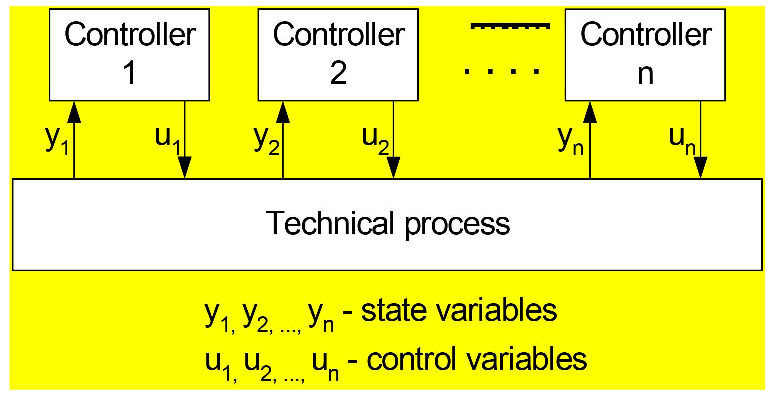
\includegraphics[width=0.48\textwidth]{figures/dezentral.pdf}
  \end{center}
  \caption{Dezentrales Kontrollsystem}
\vspace{-10pt}
\end{wrapfigure}
Das ist ein Beispieltext. 
\vspace{0.5cm}

\textbf{Zentrales Kontrollsystem}
\\
\begin{wrapfigure}{r}{0.5\textwidth}
\vspace{-20pt}
  \begin{center}
    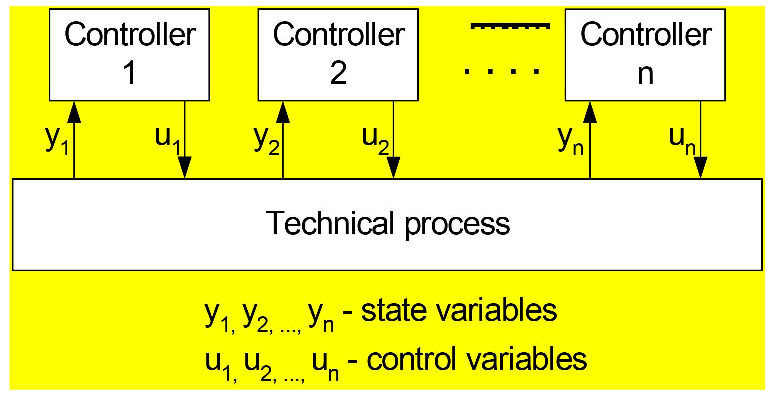
\includegraphics[width=0.48\textwidth]{figures/dezentral.pdf}
  \end{center}
  \caption{Dezentrales Kontrollsystem}
\vspace{-10pt}
\end{wrapfigure}
\textbf{Mehrebenen-Kontrollsystem}
\\
\begin{wrapfigure}{r}{0.5\textwidth}
\vspace{-20pt}
  \begin{center}
    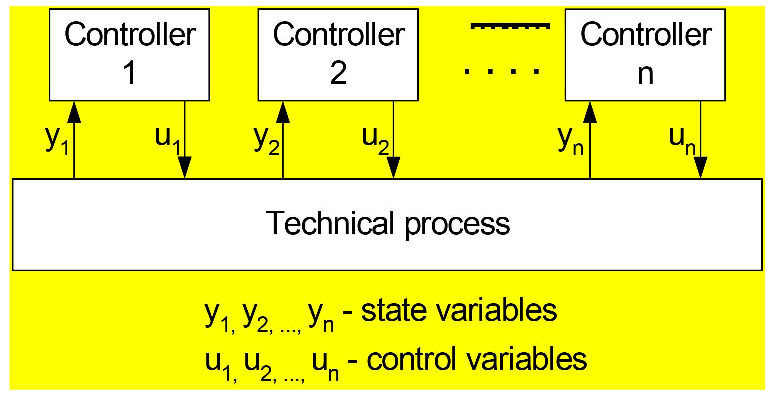
\includegraphics[width=0.48\textwidth]{figures/dezentral.pdf}
  \end{center}
  \caption{Dezentrales Kontrollsystem}
\vspace{-10pt}
\end{wrapfigure}\textbf{Netzwerkbasiertes verteiltes Kontrollsystem}
\\
\begin{wrapfigure}{r}{0.5\textwidth}
\vspace{-20pt}
  \begin{center}
    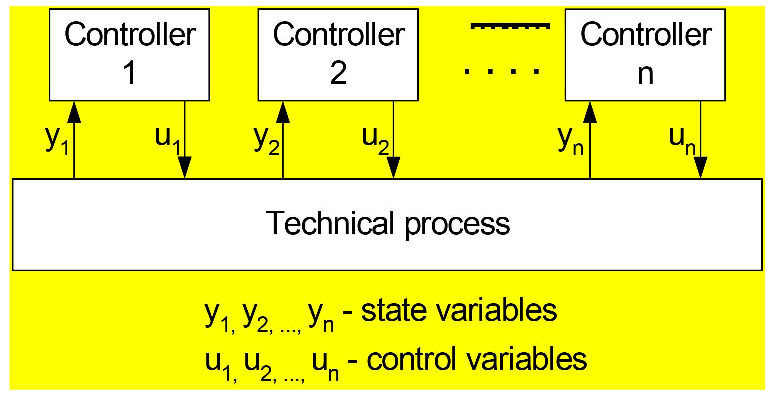
\includegraphics[width=0.48\textwidth]{figures/dezentral.pdf}
  \end{center}
  \caption{Dezentrales Kontrollsystem}
\vspace{-10pt}
\end{wrapfigure}


\pagebreak


\section{Aufgabe 4}
\begin{framed}
\textbf{Prozess-Schnittstellen} \\
Welche Vorgänge sind notwendig, um ein kontinuierliches analoges Signal in einem digitalen Computer verarbeiten zu können?
Beschreiben Sie diese und erläutern Sie die Unterschiede, wenn als Verarbeitungseinheit eine SPs oder ein Mikrocontroller verwendet wird. 
\end{framed}
\pagebreak




\section{Aufgabe 5}
\begin{framed}
\textbf{Sensorik} \\
Benennen Sie je 3 mögliche Sensoren aus dem Bereich Fahrzeug, Digitalkamera und Raumfahrt. Ordnen Sie die Wichtigkeit der Sensordaten nach ihrer Bedeutung in Bezug auf ein sicheres Funktionieren des Systems. Analysieren sie, ob analoge/digitale bzw. kontinuierliche/diskrete Signale geliefert werden und geben sie mögliche Vor- und Nachbearbeitungsschritte an. 
\end{framed}

\pagebreak

\section{Aufgabe 6}
\begin{framed}
\textbf{Speicher Programmierbare Steuerung / SPS} \\
Entwerfen sie ein SPS-Programm in zwei der standardisierten Sprachen (AWL,FBS und KOP) zur Addition zweier digitaler Eingänge A und B. Die beiden Ausgänge (Summe S und Überlauf C) sollen durch einfache logische Operationen gebildet werden. Eine Liste der möglichen Operationen ist in den VO-Folien enthalten.
\end{framed}
   
\begin{figure}[h!]
\centering
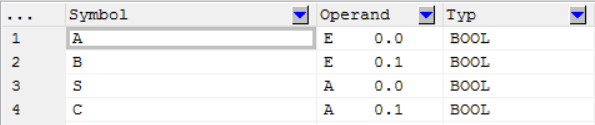
\includegraphics[scale=1]{figures/Aufg6_EA.png} 
\caption{Definition der Ein/Ausgänge}
\end{figure}

\begin{figure}[h!]
\centering
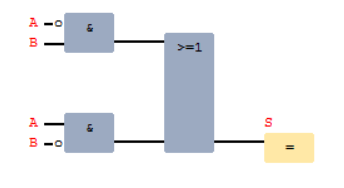
\includegraphics[scale=1]{figures/Aufg6_S_FUP.png} 
\caption{Berechnung der Summe S in Funktionsbausteinsprache FBS}
\end{figure}

\begin{figure}[h!]
\centering
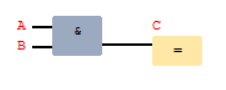
\includegraphics[scale=1]{figures/Aufg6_C_FUP.png} 
\caption{Berechnung des Übertrages C in Funktionsbausteinsprache FBS}
\end{figure}

\begin{figure}[h!]
\centering
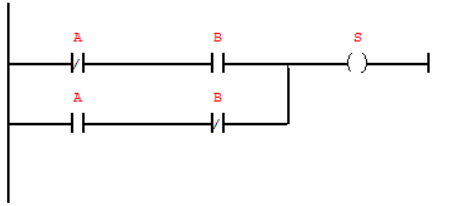
\includegraphics[scale=1]{figures/Aufg6_S_KOP.png} 
\caption{Berechnung der Summe S in Koppelplan KOP}
\end{figure}

\begin{figure}[h!]
\centering
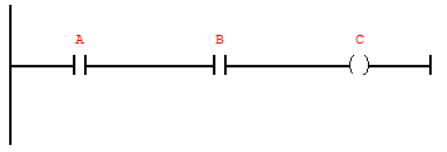
\includegraphics[scale=1]{figures/Aufg6_C_KOP.png} 
\caption{Berechnung des Übertrages C in Koppelplan KOP}
\end{figure}

\pagebreak

\section{Aufgabe 7}

\begin{framed}
\textbf{ADC im Mikrokontroller} \\
Suchen Sie sich ein Datenblatt des \textit{PIC16F1789} Mikrocontrollers. Identifizieren und beschreiben sie die Verarbeitungsmethode des eingebauten ADCs. Welche Kenngrößen werden zum Vergleich von ADCs verwendet? Bestimmen sie diese für obigen Mikrocontroller. 
\end{framed}   
   
   
   
\end{document}